
\section{Slow Starburst in the Milky Way} 
\label{bursts:sec:slowburst} 

\begin{figure*} % fig 11 
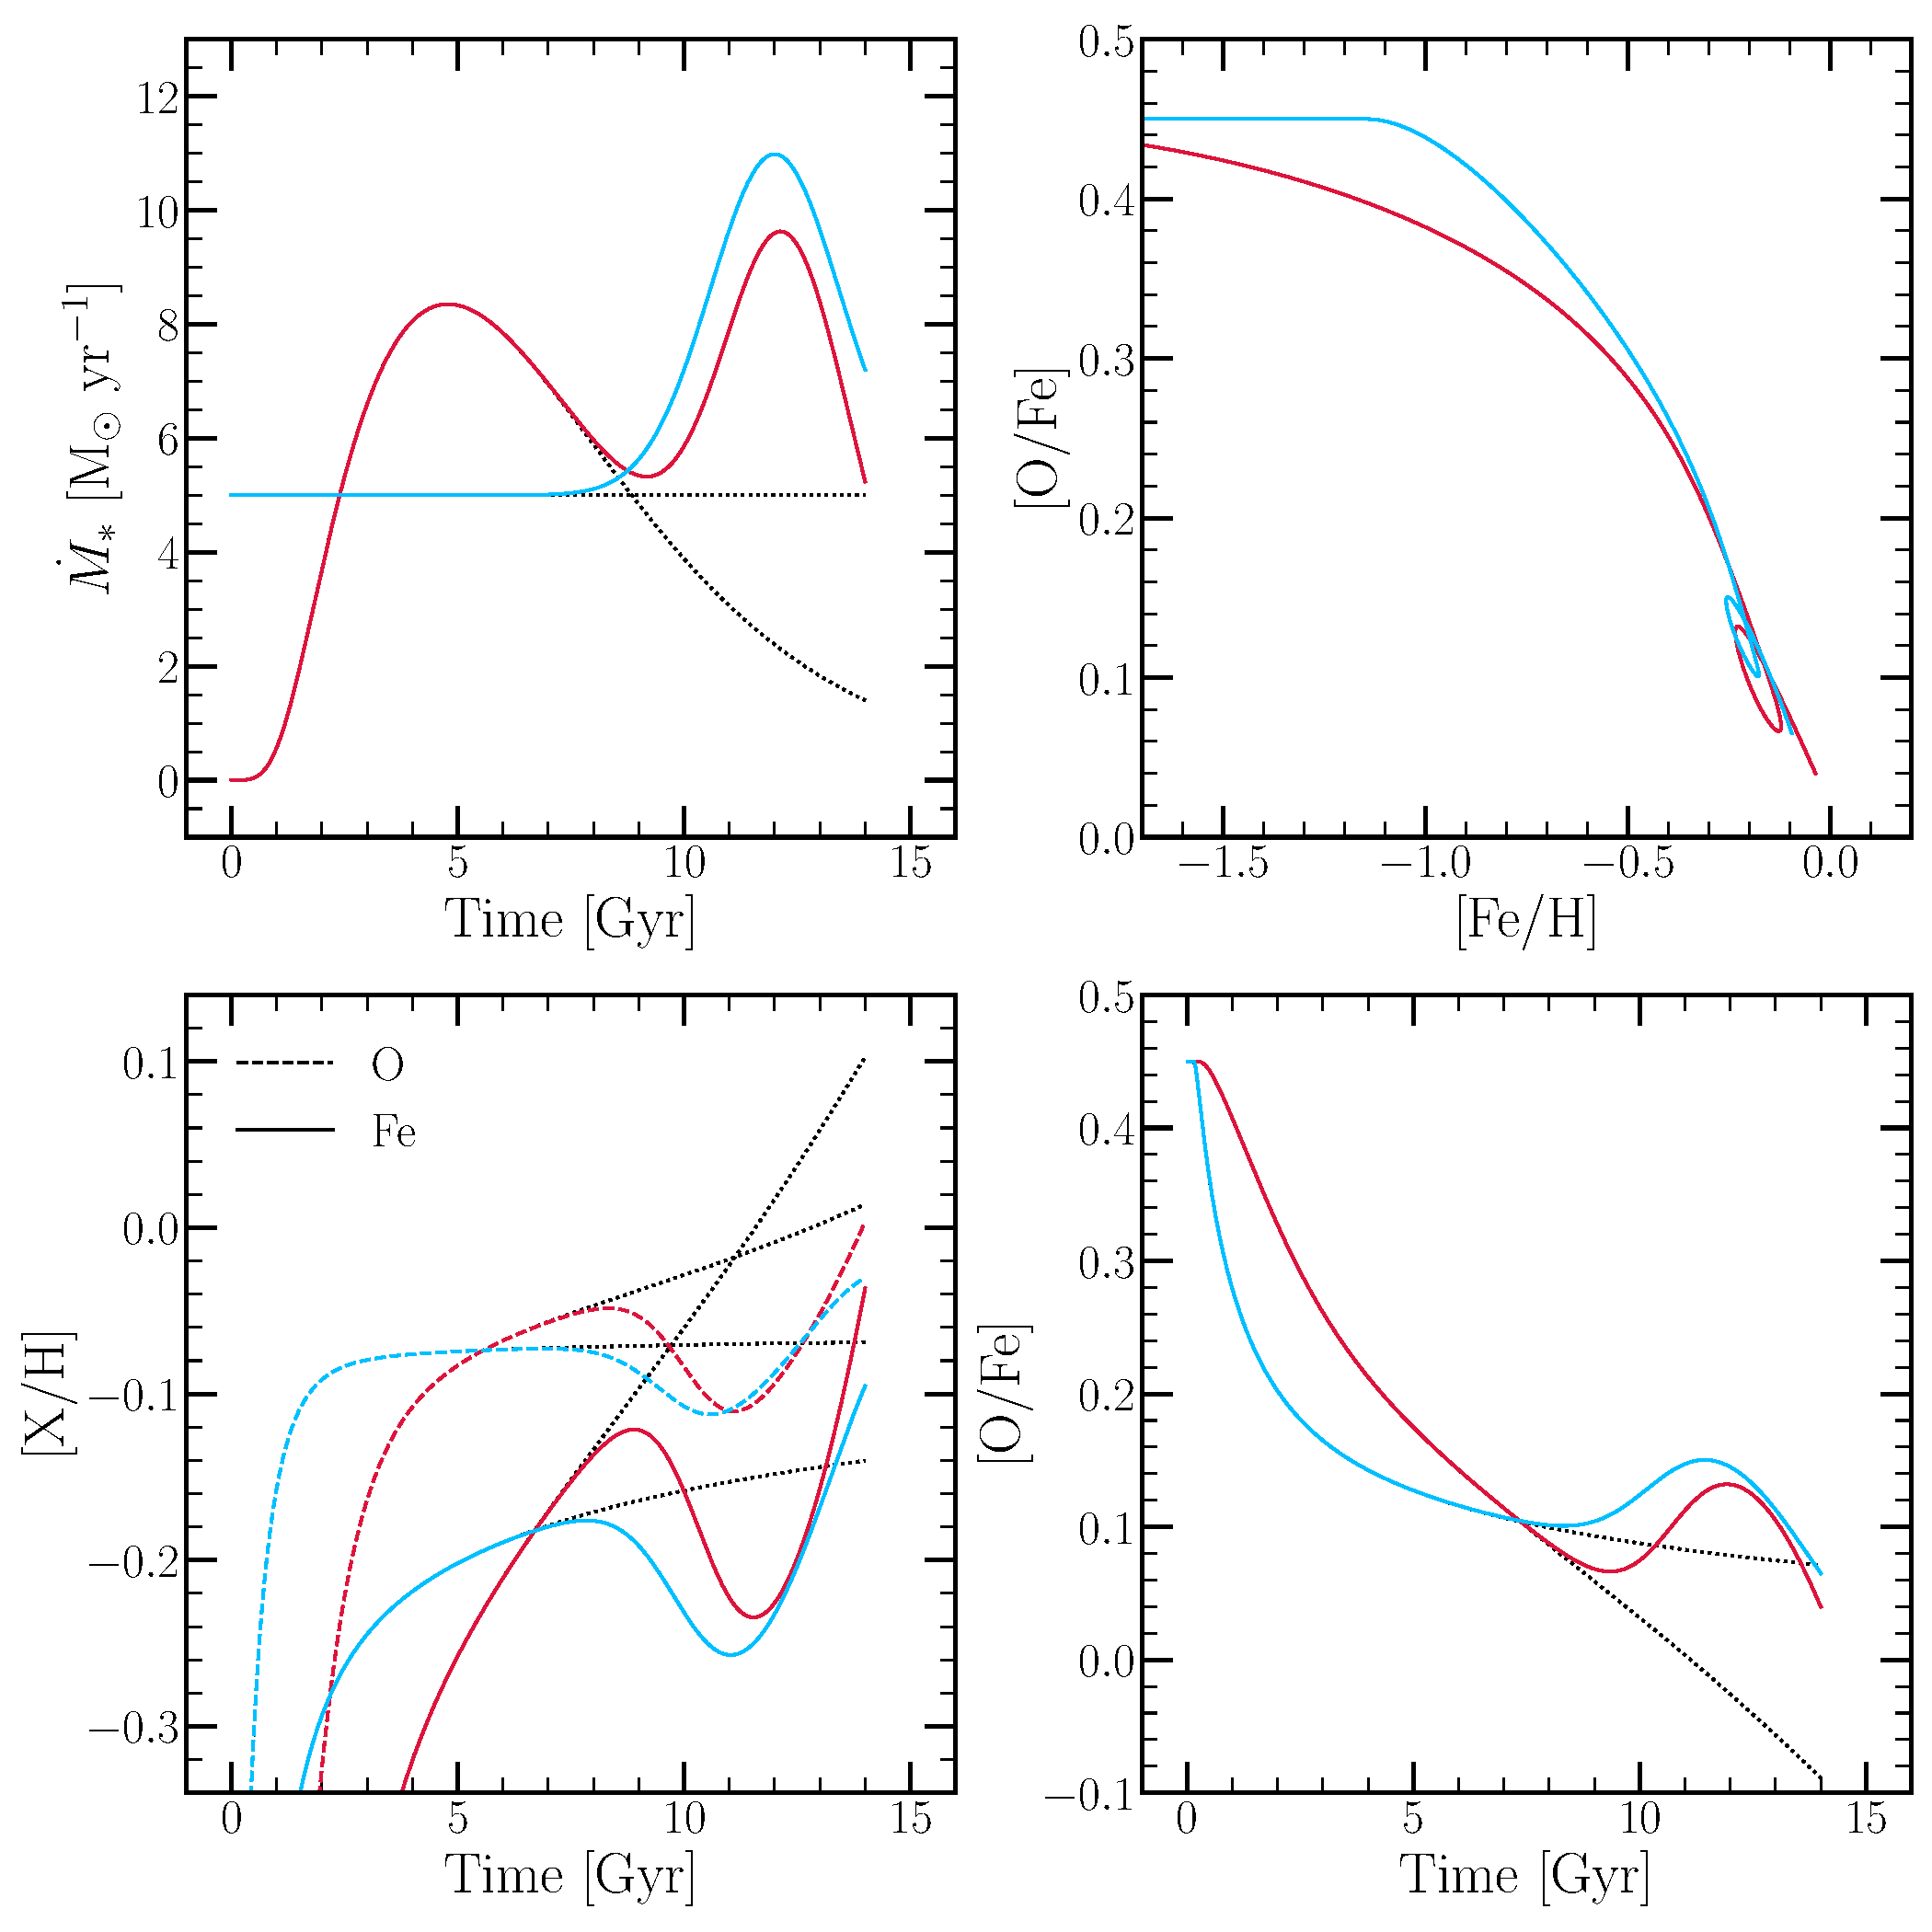
\includegraphics[scale = 0.4]{slow_bursts.pdf} 
\caption{
Models loosely motivated by recent findings of a slow starburst in the Milky 
Way~$\sim$2 Gyr ago~\citep{Mor2019, Isern2019}. These models exhibit a 
constant SFR (blue) and a $\propto t^2e^{-t}$ infall history (red), to which 
we add a Gaussian centered at $t$ = 12 Gyr with dispersion $\sigma$ = 1 Gyr to 
both models, roughly doubling the SFR at its peak. Black dotted lines in all 
panels show the corresponding quiescent scenario, to which we add no starburst. 
\textbf{Top Left}: The SFR as a function of time. 
\textbf{Top Right}: The [O/Fe]-[Fe/H] tracks. We omit the tracks of the 
quiescent model from this panel for clarity. 
\textbf{Bottom Left}: [O/H] (dashed) and [Fe/H] (solid) as a function of time. 
\textbf{Bottom Right}: [O/Fe] as a function of time. 
These models produce mildly $\alpha$-enhanced stars with young ages and a low 
median age of stars near solar metallicity. 
} 
\label{bursts:fig:slow_bursts} 
\end{figure*} 

Although our starburst models are most obviously relevant to dwarf galaxies 
with episodic star formation histories, some recent observations suggest that 
the Milky Way itself experienced substantially elevated star formation 2-3 Gyr 
ago. \citet{Mor2019} infer such a history by comparing population synthesis 
models to observed stellar luminosity functions and color-magnitude diagrams 
from Gaia data. \citet{Isern2019} reaches similar conclusions from modeling the 
luminosity function of white dwarfs in the solar neighborhood measured using 
Gaia parallaxes. Although these white dwarfs are close to the sun, dynamical 
mixing implies that they at least sample the history of the solar annulus, 
and older white dwarfs likely sample a range of galactocentric radii because of 
radial mixing. Resolved stellar population studies of the M31 disk also provide 
evidence for elevated star formation 2-4 Gyr ago with much lower SFR before 
and after~\citep[][Figs. 22-23]{Williams2017}. 
\par 
Fig.~\ref{bursts:fig:slow_bursts} presents the evolution of two models loosely 
motivated by these observations. The first (blue curves) has a constant SFR to 
which we have added a burst described by a Gaussian centered at $t = 12$ Gyr 
(lookback time 2 Gyr) with dispersion of 1 Gyr. At its peak, this burst 
approximately doubles the galaxy SFR relative to the pre-burst value. The 
second model (red curve) adds a similar burst to a model with an infall 
history described by $\dot{M}_\text{in} \propto t^2e^{-t}$ with $e$-folding 
timescale $\tau_\text{inf} = 2.2$ Gyr. The pre-burst SFR first climbs as the 
gas supply builds (starting from zero), then declines as the infall rate slows. 
The qualitative appearance of this model is similar to those in Fig. (1) 
of~\citet{Isern2019}. For both models we adopt $\eta$ = 2.5 and 
$\tau_* = (\text{2 Gyr})(M_\text{g}/6.0\times10^9\ M_\odot)^{-0.5}$, allowing 
\texttt{VICE} to solve for the infall rate required to produce the starburst. 
We also plot the evolution of the corresponding quiescent models in dotted 
lines for comparison; they follow the same evolution but with no added 
starburst. 
\par 
The [O/Fe]-[Fe/H] tracks show loops similar to those of our infall-driven and 
efficiency-driven burst models (e.g., Fig.~\ref{bursts:fig:fiducial_cases})
and qualitatively resemble that of~\citet{Spitoni2019}, who investigated 
similar models for the solar annulus in much greater detail. 
As found 
in previous studies~\citep{Andrews2017, Weinberg2017b}, the exponential 
infall model exhibits slower pre-burst evolution and a more gradual ``knee'', 
and because of the short $e$-folding timescale even the unperturbed model does 
not approach equilibrium by $t$ = 14 Gyr. The critical feature of these models 
relative to our fiducial starbursts is that the effects of the bursts have not 
decayed by the end of the simulations at $t$ = 14 Gyr. Over the final 2 Gyr, 
the values of [O/H] and [Fe/H] are rapidly climbing and end at values higher 
than those reached at any previous time. The [O/Fe] values in both models 
reach a local maximum at $t$ = 12 Gyr, then fall for the final 2 Gyr. 
\par 
These results are of particular interest in light of recent 
studies of age-abundance relations from the Apache Point Observatory Galaxy 
Evolution Experiment (APOGEE)~\citep[e.g.][]{Martig2016,
SilvaAguirre2018, Feuillet2018, Feuillet2019}. The late bump in [O/Fe] could 
help explain populations of young $\alpha$-enhanced stars~\citep{Martig2016, 
Feuillet2019}, though in these models such stars would have modest 
$\alpha$-enhancements, 
near-solar metallicity, and age $\approx$ 2 Gyr. The late-time bumps in [O/H] 
and [Fe/H] could help to explain the strikingly young (1-2 Gyr) median ages that 
\citet{Feuillet2018} find for solar neighborhood stars with [Fe/H] $\approx$ 
0 or [O/H] $\approx$ 0. Finally, the most $\alpha$-poor stars predicted by 
these models form at late times in the wake of the burst, potentially 
explaining the low median age ($\sim$1 Gyr) that~\citet{Feuillet2018} find for 
stars with [$\alpha$/Fe] < 0. The age-metallicity relation 
for solar neighborhood stars exhibits large scatter~\citep{Edvardsson1993}, 
and explaining this scatter likely requires radial mixing of stellar 
populations~\citep[e.g.][]{Schoenrich2009a} or some other mechanism not 
represented in one-zone GCE models. However, while multi-zone models with 
radial mixing and smooth star formation histories can explain a large 
dispersion in age-abundance relations, they still have difficulty reproducing 
the young median ages inferred for solar metallicity stars~\citep[][see 
their Fig. 15]{Feuillet2018}. 
The one-zone models presented here suggest that elevated star formation in the 
recent past could have a significant impact on age-abundance relations, 
pushing them away from the equilibrium behaviour predicted for smooth star 
formation histories. Furthermore, the differences between these models and 
their corresponding quiescent cases at late times raise the intriguing 
possibility that the recent burst in the Milky Way has not yet fully decayed. 
This would imply that the present day chemistry of the Milky Way is still 
mildly perturbed due to the recent starburst. We reserve an exploration of 
models combining radial mixing with star formation histories like those 
of~\citet{Mor2019} and~\citet{Isern2019} for future work.

